\documentclass[]{elsarticle} %review=doublespace preprint=single 5p=2 column
%%% Begin My package additions %%%%%%%%%%%%%%%%%%%
\usepackage[hyphens]{url}

  \journal{An awesome journal} % Sets Journal name


\usepackage{lineno} % add
\providecommand{\tightlist}{%
  \setlength{\itemsep}{0pt}\setlength{\parskip}{0pt}}

\usepackage{graphicx}
\usepackage{booktabs} % book-quality tables
%%%%%%%%%%%%%%%% end my additions to header

\usepackage[T1]{fontenc}
\usepackage{lmodern}
\usepackage{amssymb,amsmath}
\usepackage{ifxetex,ifluatex}
\usepackage{fixltx2e} % provides \textsubscript
% use upquote if available, for straight quotes in verbatim environments
\IfFileExists{upquote.sty}{\usepackage{upquote}}{}
\ifnum 0\ifxetex 1\fi\ifluatex 1\fi=0 % if pdftex
  \usepackage[utf8]{inputenc}
\else % if luatex or xelatex
  \usepackage{fontspec}
  \ifxetex
    \usepackage{xltxtra,xunicode}
  \fi
  \defaultfontfeatures{Mapping=tex-text,Scale=MatchLowercase}
  \newcommand{\euro}{€}
\fi
% use microtype if available
\IfFileExists{microtype.sty}{\usepackage{microtype}}{}
\bibliographystyle{elsarticle-harv}
\ifxetex
  \usepackage[setpagesize=false, % page size defined by xetex
              unicode=false, % unicode breaks when used with xetex
              xetex]{hyperref}
\else
  \usepackage[unicode=true]{hyperref}
\fi
\hypersetup{breaklinks=true,
            bookmarks=true,
            pdfauthor={},
            pdftitle={Practical Applications for a Distributed Modeling Framework for Protected Data},
            colorlinks=false,
            urlcolor=blue,
            linkcolor=magenta,
            pdfborder={0 0 0}}
\urlstyle{same}  % don't use monospace font for urls

\setcounter{secnumdepth}{0}
% Pandoc toggle for numbering sections (defaults to be off)
\setcounter{secnumdepth}{0}

\newlength{\cslhangindent}
\setlength{\cslhangindent}{1.5em}
\newenvironment{cslreferences}%
  {\setlength{\parindent}{0pt}%
  \everypar{\setlength{\hangindent}{\cslhangindent}}\ignorespaces}%
  {\par}

% Pandoc header



\begin{document}
\begin{frontmatter}

  \title{Practical Applications for a Distributed Modeling Framework for
Protected Data}
    \author[Johns Hopkins Bloomberg School of Public Health]{John
Muschelli III\corref{Corresponding Author}}
   \ead{jmusche1@jhu.edu} 
      \address[Johns Hopkins Bloomberg School of Public
Health]{Department of Biostatistics, 615 N Wolfe St, Baltimore MD,
21205}
    
  \begin{abstract}
  We present 2 practical approaches to fitting generalized linear models
  in a distributed framework. The use case for this framework is where
  multiple sites (e.g.~hospitals) have data with protected or private
  information that cannot be shared, but aggregated data can be, and
  each site can send aggregated data across the internet.\\
  We present the first strategy: using synced folder services, such as
  Dropbox or Box Sync, to share the aggregated data. The second strategy
  involves creating an application programming interface (API), where
  sites submit the data to this service. This work relies on the R
  statistical software; we provide an R package of examples and code to
  create an API on DigitalOcean.
  \end{abstract}
  
 \end{frontmatter}

\hypertarget{introduction}{%
\section{Introduction}\label{introduction}}

We introduce a distrbuted framework to analyze data from multiple
sources with the data being properly siloed. The motivation for this
problem is simple: we would like to fit a generalized linear model (GLM)
on data from multiple sites (e.g.~hospitals), where the indvidual
patient-level data or otherwise private data never leaves the server
(siloed), which is usually behind a firewall. The idea is that a model
is specified, and sent to each site where a summary statistic is
computed and returned to the modeling service/site. The model is then
updated and, if necessary, the process is completed until the model is
fit until convergence. The goal is to fit the exact model as if the full
data was accessible.

The alternatives to this process is meta-analysis, one-step solutions,
or remote analysis servers {[}O'Keefe and Good (2008);{]}. There are
drawbacks to a meta-analysis approach in that the model and statistics
must be specified and commonly the data is gathered \textbf{once} from
each site. Also, if sites present estimates from models with different
predictors, it is unclear how meta-analysis adequately handles this
variability. The process below ensures that the same model, with the
same predictors, is fit at each site. Any updated analysis requires
additional correspondence between the modeler and the site data analyst,
which slows down the process of analysis and creates more hurdles.

The work presented here is almost identical to Grid Binary LOgistic
REgression (GLORE) (Wu et al., 2012), its Bayesian analog EXpectation
Propagation LOgistic REgRession (EXPLORER) (Wang et al., 2013), and
Secure Pooled Analysis acRoss K-sites (SPARK) (El Emam et al., 2013). A
few of the differences are: GLORE and EXPLORER focus primarily on only
logistic regression, SPARK works for all GLMs like the proposed method.
GLORE and SPARK are iterative requiring all sites to provide updates
until the next estimate can be achieved, like the current method;
EXPLORER is iterative but asynchronous so that sites can share updates
without coordination. SPARK additionally compute on encrypted data,
which allows for higher security; EXPLORER uses random matrix
implementations to increase security, but required inter-site
communication. Similarly, Wang et al. (2017) show an iterative method
for regularized/sparse model fitting. Jordan et al. (2019) present a
general framework by sending surrogate likelihood information in an
iterative way, which generalizes over GLMs, and they examples of
M-estimators, regularized/penalized models, and Bayesian models. All
previous solutions do not provide practical steps or tutorials to set up
a system, however.

To alleviate the need for iterative processes, one-shot solutions have
been presented. For example, One-shot Distributed Algorithm to perform
Logistic regressions (ODAL) (Duan et al., 2019) is a distributed
estimation procedure for a logistic model. for a given \(\beta\),
compute gradients of a likelihood and use these computed gradients to
inform the estimate of \(\beta\), but only with one iteration. They have
shown to get close estimates to the ``true model'', which would be the
model fit if all data was included. The work is expanded upon in
Robust-ODAL (Tong et al., 2020), where median gradients are estimated as
opposed to mean gradients, to diminish the influence of heterogeneous
site data. Other methods have shown that efficient one-step estimators
or averages perform well compared to an ``oracle model'' with the full
data (Battey et al., 2018; Zhang et al., 2013). These methods provide
great approximate solutions because 1) they are not iterative, 2) can be
computed in a privacy-preserving way, 3) can be robust to outlying data,
and 4) can be seen as likelihood updates. As a likelihood update, the
same process can be done with all but one site, determining the
robustness of the procedure in a sensitivity analysis. The downsides are
that the solution is approximate and if another model is to be run, the
whole process has to start again. Thus, we believe a remote analysis
server can be more general.

The work presented here is similar to that of O'Keefe and Good (2009) as
it has a remote analysis server, but with a main difference. Practical
implementations such as WebDISCO (web service for distributed Cox model
learning) exist, but these rely on a third-party service (at this time
the WebDISCO URL is a dead link) or a remote analysis server. In O'Keefe
and Good (2009) and most remote analysis servers, a full dataset
primarily exists. That is, the full data is available to that server,
but not those submitting the models.

The most common federated learning architecture is Federated Averaging
(McMahan et al., 2016), which uses stochastic gradient descent to
combine neural network parameters from multiple devices into one
platform. Many platforms have been developed for this type of federated
learing, such as Federated Learning platform from Google for deep
learning (Bonawitz et al., 2019), Content Object Repository Discovery
and Registration/Resolution Architecture (CORDA), which website does not
seem to be associated with the platform anymore). Geyer et al. (2017)
and https://comind.org/ provide code on how to set up clients and run a
federated deep learning model, but we wish to focus on simpler GLMs in
this work, but acknowledge similar inference could be reframed in work
based on Tensorflow. Li et al. (2019) provides an overview of federated
learning

Moreover, some remote analysis servers may be complicated and costly to
set up or have little to no instruction on how to set them up, save for
the examples with code above. We will present a system that does have
the same constraints, as it will rely on a few scripts or spooling up on
a server on a low-cost online service with one command.

We are not experts in distributed/federated computing, but would like to
show how this process is possible, overlooking obvious hurdles such as
authentication, load balancing, network issues, debugging, and overall
security on the server side. That said, some of the previous methods and
authors present solutions with a series of additional checks with
privacy-preserving measures which can be implemented. We argue that
analysts already have this responsibility of security, but in a more
informal way. In some of the applications above, such as some of the
one-shot solutions, the model specification and updates are communicated
by easy, likely unsecure methods such as email. Thus, it would seem as
though iterative methods can give exact solutions in a secure way, but
the iterative process is burdensome, and one-shot solutions are
user-friendly but potentially as insecure as the proposed method. We
wish to make the iterative process easy and user-friendly.

A large reason for the importance of usuability is that the
statisticians and data analysts that will be running the models will
likely be using a statistical language, usually either R or Python.
Though we will focus on R, the ideas here can be extended to other
languages and systems (R Core Team, 2020). We implemented a practical
solution in an R package that allows researchers to practically
implement this system with real data. The solution can be done a number
of ways; we implemented 1) code to deploy an API (application
programming interface) on a remote server and 2) scripts to calculate
the model if using a synced folder, backed by services such as Dropbox
or Box Sync. This practical solution solves the motivating problem,
allowing us to fit many different types of models with little technical
overhead while keeping protected health information (PHI) private.

\hypertarget{methods}{%
\section{Methods}\label{methods}}

\hypertarget{motivating-example}{%
\subsection{Motivating Example}\label{motivating-example}}

Let's estimate a GLM an outcome \(Y\) on a set of covariates \(X\), with
a link function \(G\). Let there be \(K\) hospitals, and \(Y\) and \(X\)
are on the data on all hospitals \(1, \dots, K\).

\[
g(E[Y | X]) = X\beta = \eta
\]

Let us also say that we are interested in \(p\) covariates, and
\(n_{k}\) is the total number of records at hospital \(k\) and
\(n = \sum_{1}^{k} n_{k}\), is the number of rows of \(Y\) and \(X\),
thus \(Y\) is an \(n\text{x}1\) vector and \(X\) is a \(n\text{x}p\)
matrix. To estimate \(\beta\), we would use: \[
(X'WX)^{-1} X'WY
\]

Since we don't have access to the full \(X\), but rather a series of
\(X_{k}\), \(k = 1, \dots, K\), we can use methods such as parallelized
gradient descent approaches (Mcdonald et al., 2009; Zinkevich et al.,
2010) or approximate maximum-likelihood approaches (Duncan, 1980). We
choose to use the Fisher scoring method outlined in McCulloch (2000)
(page 42), such that:

\[
u_{i,k} = \sum W (y_{i,k} - \mu) \frac{d\eta}{d\mu}x_{i,k}
\] where we will get \(u_{k} = \sum_{i} u_{i, k}\) and \[
W^{-1} = \left(\frac{d\eta}{d\mu}\right)^2V
\] where \(V\) is the variance function for the GLM evaluated at
\(\mu\). If we let \(A_{k} = X_k'W_kX_k\) we can get
\(A = \sum_{k}A_{k}\), which is a \(p\text{x}p\) matrix. If we get
\(u_{k}\), which is a \(p\times 1\) vector, then we can calculate
\(u = \sum_{k} u_{k}\) to get the necessary gradient \(\nabla\beta\) by
\(A^{-1} u\). To estimate the dispersion parameter \(\phi\), we need the
sample size for each site \(n_{k}\) and the sum of squared residuals,
which each are a scalar number. Thus, for generalized linear models, we
need only to pass a \(p\times{p}\) matrix \(A\) and \(p\times{1}\)
vector \(u\), and 2 scalar values from each site.

\hypertarget{implementation}{%
\subsection{Implementation}\label{implementation}}

We provide the \texttt{distribglm}
(https://github.com/muschellij2/distribglm) R package to perform the
distributed learning models. The functions provided wherein allow for
the fitting of models in addition to 2 specific sets of examples: a
\texttt{plumber} file and a set of examples files using a ``synced
folder''.

\hypertarget{synced-folder-implementation}{%
\subsubsection{Synced Folder
Implementation}\label{synced-folder-implementation}}

Example synced folders are Dropbox or Box Sync. Outside of the R
package, all sites would have access to a synced folder. This folder
will only contain information about the model specifications and the
estimates above. \textbf{No PHI would go in this folder}, as it is
shared across sites and the main compute site, which may be a
data-sharing site.

The first step in the process is to set up the model (with the
\texttt{setup\_model} function), which requires the synced folder
location, the generalized linear model formula, which exponential family
(and link function) is to be fit, a model name, the identifiers for all
the sites to use for this model, and an optional tolerance measure that
defines when a model has converged. The site identifiers are necessary
for bookkeeping as well as to notify the compute site when all sites
have returned the updated statistics for aggregation and provides a
notification to each site as to whether the process is waiting on other
sites or the compute site.

Once this function is run, the output file is synced across all sites
and the compute site. The data sites then run \texttt{estimate\_model}
at the same time and the compute site runs \texttt{compute\_model}.
Again, as these updates are required to be synchronous, these have to be
run at the same time. We believe a simple conference call walking
through each step is a practical example of when this would occur. Each
site must change the code to read in the data (from a different location
than the synced folder) into R, provide the site name, and the location
of the synced folder on their machine, as this may vary across
sites/computers. The data set will have its rows shuffled and the
parameters estimated and only the parameter information will be sent.

Once finished, the model will be returned and saved. At that point, all
iterations could be deleted or archived.

\hypertarget{plumber-implementation}{%
\subsubsection{Plumber Implementation}\label{plumber-implementation}}

\texttt{plumber} is an R package that creates APIs (Application
programming interfaces) for and from R (Trestle Technology, LLC, 2018).
Though there are many frameworks to create APIs, such as Node.js and
Flask, we will focus on \texttt{plumber} for a number of reasons.
Overall, the API needs a computational backbone for this process to
work. As \texttt{plumber} is based in R, we know that the server will
have this already installed. The function
\texttt{do\_provision\_glm\_api} will provision a DigitalOcean
(https://www.digitalocean.com/) ``droplet'', which is an instance of a
running virtual machine on a server. This will install R on the server,
web services such as \texttt{nginx}, \texttt{plumber}, and all the
necessary R packages to perform the distributed computing.

The process is similar as above, but the need for a ``compute site'' is
now replaced by the API. The additional parameter required is the URL to
the API endpoint, which will be given to each site. A modeler or someone
to specify the model is still required, which would use
\texttt{api\_setup\_model} with the same information as above. The model
then would make the same folder structure as in the synced folder
implementation above. The sites would then run
\texttt{api\_estimate\_model}, which would pass in the data the same
way, and send the same information as above, but again requiring the URL
of the API to be passed in for both functions. Additional login
information and API keys can be set up so that more formal
authentication can be performed

\begin{figure}
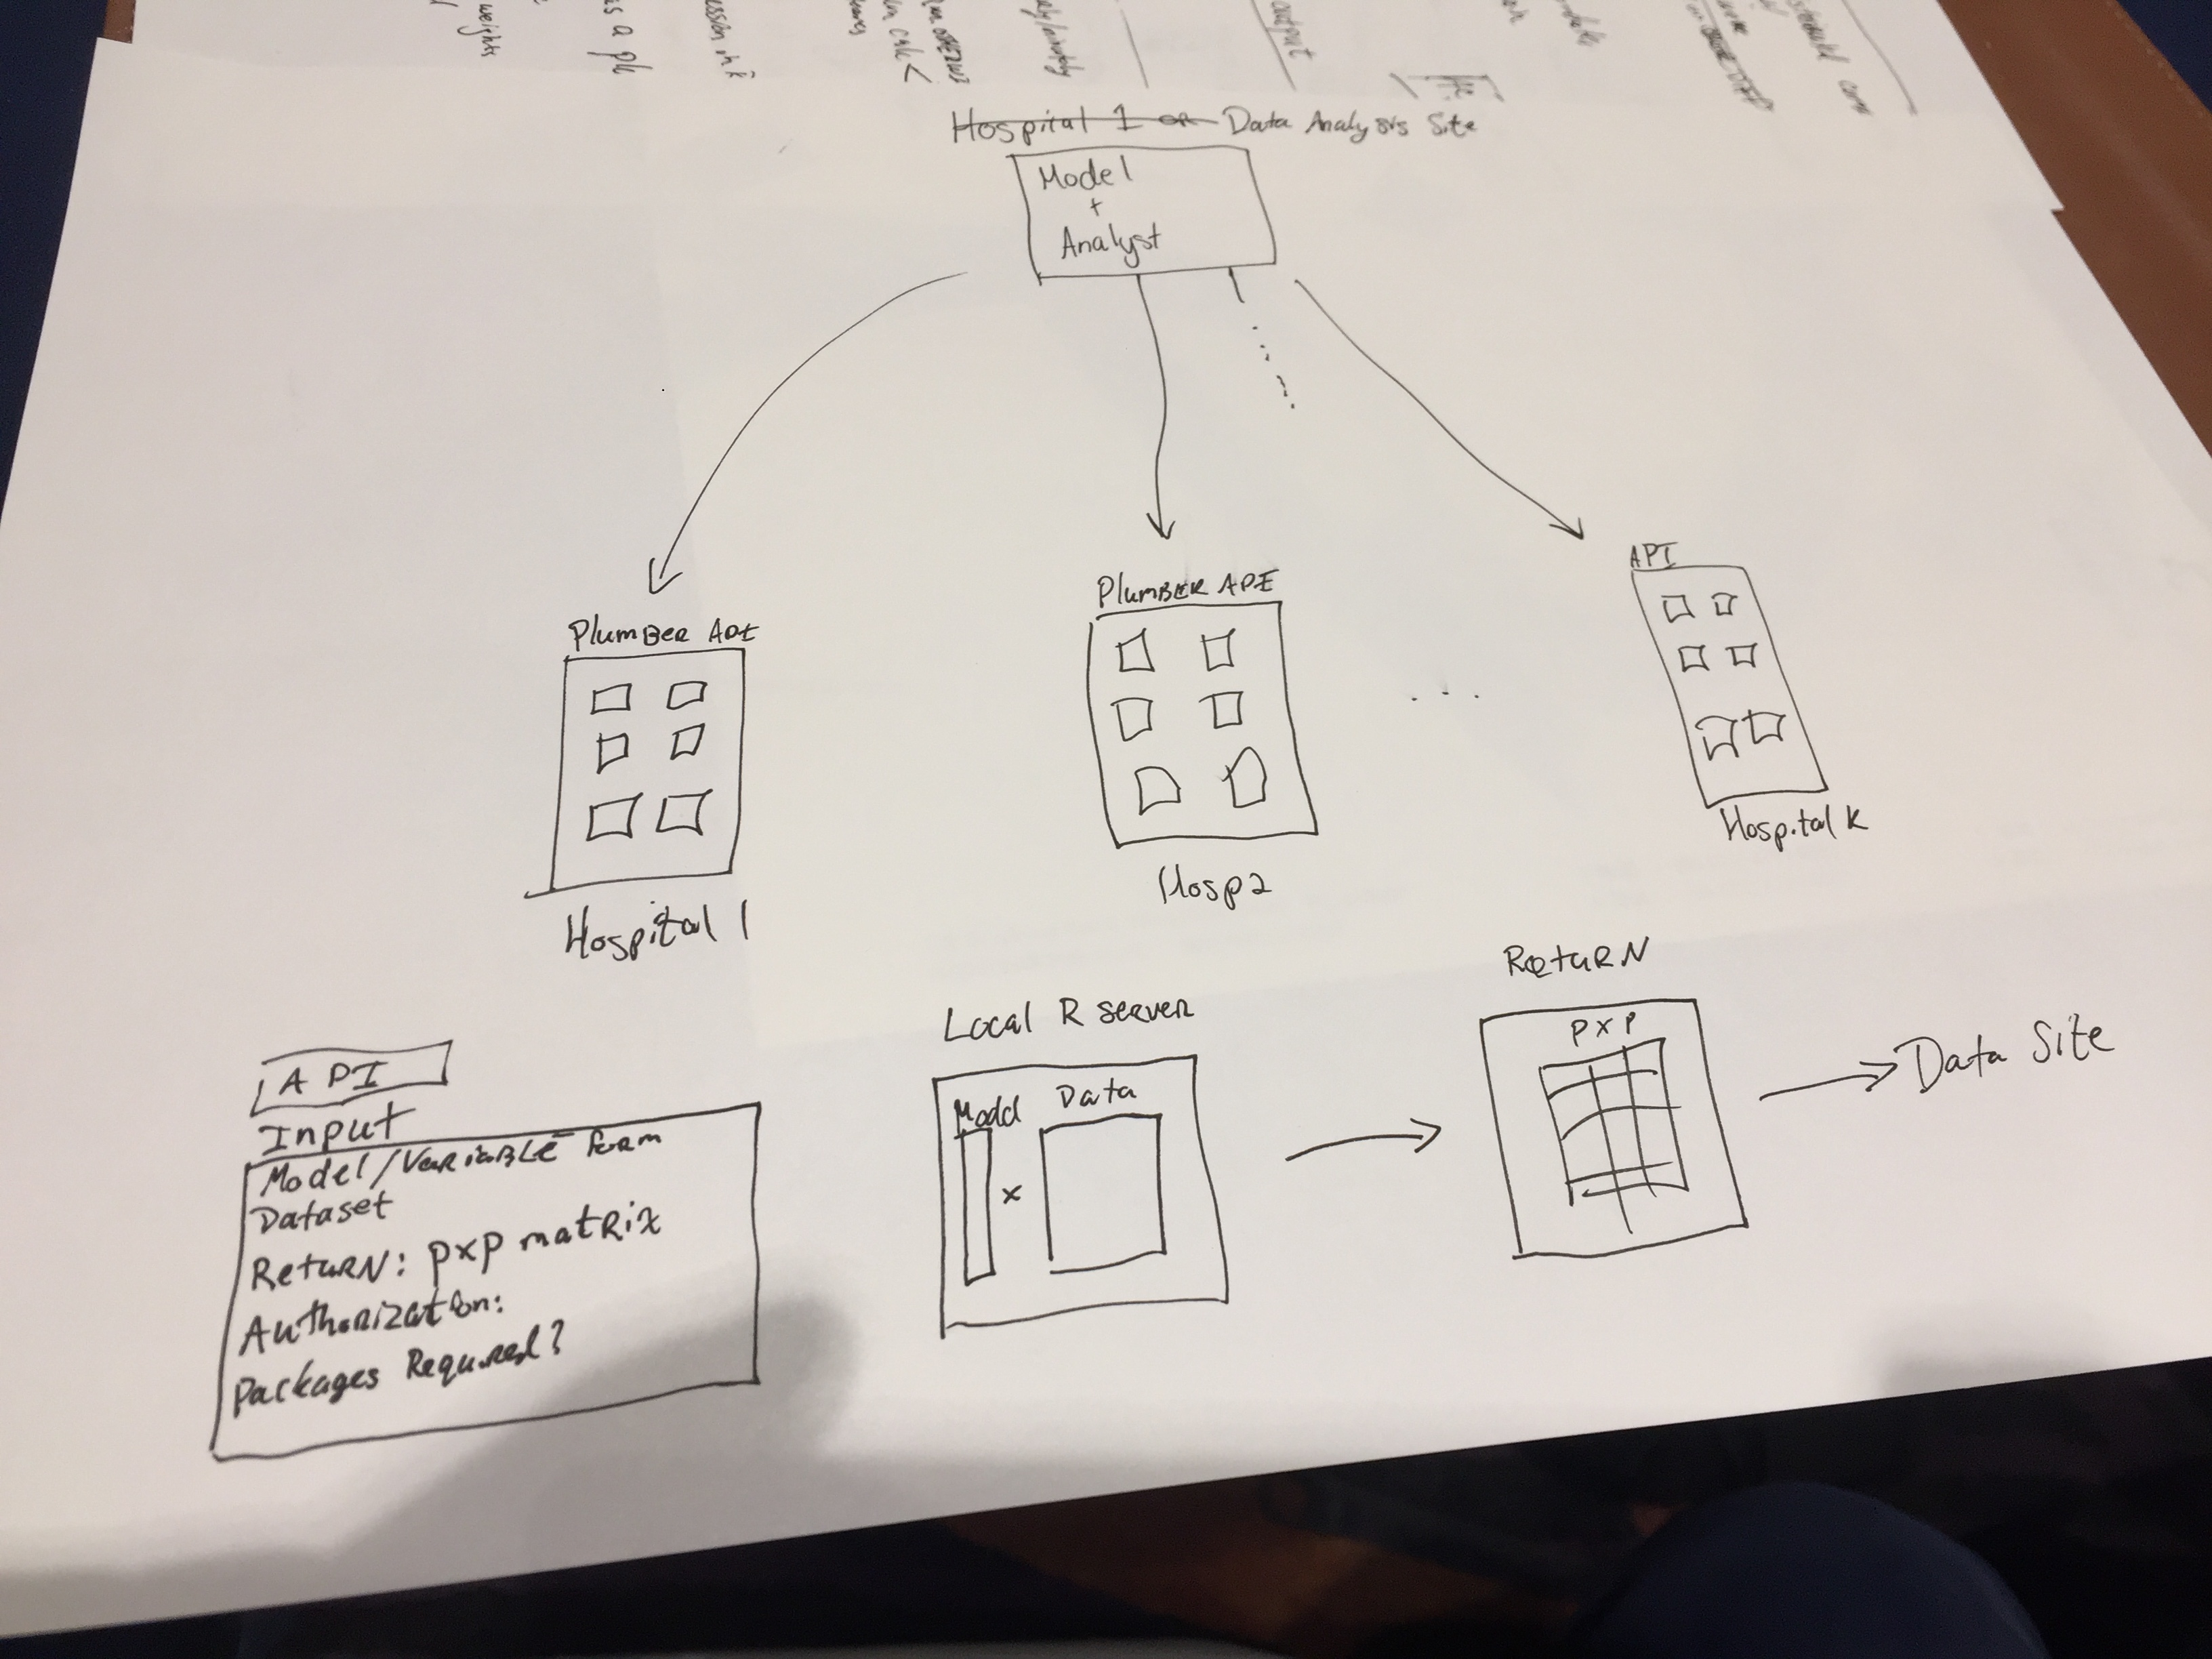
\includegraphics[width=1\linewidth]{sketch} \caption{Proposed Framework.  The modeler/analyst specifies a model, sends the model specification to an endpoint on each hospital API, a computation is run and returned to the analyst and aggregated (usually a gradient).  The model estimates are updated and the process repeats until the model converges.  }\label{fig:unnamed-chunk-1}
\end{figure}

\hypertarget{results}{%
\subsection{Results?}\label{results}}

\hypertarget{issues}{%
\section{Issues}\label{issues}}

Though the system may seem simple to describe, many obstacles exist.
Mainly opening any system that interacts with patient data or a database
(even if it were a spreadsheet) is a potential security risk which most
clinical centers will not allow. Though this caution is warranted, it
may be more secure than the alternative of sending estimates in other
communication systems such as email. Though emailing has the upside of a
human ensuring only aggregate data is transferred, it drastically
increases the potential for wrong computation. For example, the
\texttt{distriblm} package can have add checks on the data for
missingness, quality, the sample size is equal to that of the previous
iteration/model, and other issues, which may be done at varying levels
at each institution.

If a user chooses the API solution, then a server is required, and
though we provide an easy solution on DigitalOcean, many institutions
choose to use their own systems, which may require an administrator to
oversee it. This administrator is usually trained in information systems
or information technology, which is likely not part of the clinical
team. Thus, providing support or interaction from the clinical team to
the technical personnel can be more costly than simply emailing
estimates. Lastly, many institutions and research groups would like a
``handle'' on what models are being fit with their data, and thus limits
on the API need to be created, which may cause other issues or
limitations on teh proposed framework.

These downsides are vastly outweighed when the system gets repeated use.
Thus, fitting one model one time does not generally warrant the work
needed to set up this framework. One specific example is running the
same model with different combinations of sites, allowing for a formal
sensitivity analysis.

Additional security requirements should like be enabled on such as
platform, such as random sub-sampling of the data at each site, adding
noise to the vectors and matrices passed so that the sum is the same but
each individual site has distorted estimates,

\hypertarget{references}{%
\section*{References}\label{references}}
\addcontentsline{toc}{section}{References}

\hypertarget{refs}{}
\begin{cslreferences}
\leavevmode\hypertarget{ref-battey2018distributed}{}%
Battey, H., Fan, J., Liu, H., Lu, J., Zhu, Z., 2018. Distributed testing
and estimation under sparse high dimensional models. Annals of
statistics 46, 1352.

\leavevmode\hypertarget{ref-bonawitz2019towards}{}%
Bonawitz, K., Eichner, H., Grieskamp, W., Huba, D., Ingerman, A.,
Ivanov, V., Kiddon, C., Konecny, J., Mazzocchi, S., McMahan, H.B.,
others, 2019. Towards federated learning at scale: System design. arXiv
preprint arXiv:1902.01046.

\leavevmode\hypertarget{ref-duan2019odal}{}%
Duan, R., Boland, M.R., Moore, J.H., Chen, Y., 2019. ODAL: A one-shot
distributed algorithm to perform logistic regressions on electronic
health records data from multiple clinical sites., in: PSB. World
Scientific, pp. 30--41.

\leavevmode\hypertarget{ref-duncan1980approximate}{}%
Duncan, G.M., 1980. Approximate maximum likelihood estimation with data
sets that exceed computer limits. matrix 2, 1.

\leavevmode\hypertarget{ref-spark}{}%
El Emam, K., Samet, S., Arbuckle, L., Tamblyn, R., Earle, C.,
Kantarcioglu, M., 2013. A secure distributed logistic regression
protocol for the detection of rare adverse drug events. Journal of the
American Medical Informatics Association 20, 453--461.

\leavevmode\hypertarget{ref-2017arXiv171207557G}{}%
Geyer, R.C., Klein, T., Nabi, M., 2017. Differentially Private Federated
Learning: A Client Level Perspective. ArXiv e-prints.

\leavevmode\hypertarget{ref-jordan2019communication}{}%
Jordan, M.I., Lee, J.D., Yang, Y., 2019. Communication-efficient
distributed statistical inference. Journal of the American Statistical
Association 114, 668--681.

\leavevmode\hypertarget{ref-li2019federated}{}%
Li, T., Sahu, A.K., Talwalkar, A., Smith, V., 2019. Federated learning:
Challenges, methods, and future directions. arXiv preprint
arXiv:1908.07873.

\leavevmode\hypertarget{ref-mcculloch2000generalized}{}%
McCulloch, C.E., 2000. Generalized linear models. Journal of the
American Statistical Association 95, 1320--1324.

\leavevmode\hypertarget{ref-mcdonald2009efficient}{}%
Mcdonald, R., Mohri, M., Silberman, N., Walker, D., Mann, G.S., 2009.
Efficient large-scale distributed training of conditional maximum
entropy models, in: Advances in Neural Information Processing Systems.
pp. 1231--1239.

\leavevmode\hypertarget{ref-mcmahan2016communication}{}%
McMahan, H.B., Moore, E., Ramage, D., Hampson, S., others, 2016.
Communication-efficient learning of deep networks from decentralized
data. arXiv preprint arXiv:1602.05629.

\leavevmode\hypertarget{ref-o2008remote}{}%
O'Keefe, C.M., Good, N.M., 2008. A remote analysis server-what does
regression output look like?, in: International Conference on Privacy in
Statistical Databases. Springer, pp. 270--283.

\leavevmode\hypertarget{ref-o2009regression}{}%
O'Keefe, C.M., Good, N.M., 2009. Regression output from a remote
analysis server. Data \& Knowledge Engineering 68, 1175--1186.

\leavevmode\hypertarget{ref-RCORE}{}%
R Core Team, 2020. R: A language and environment for statistical
computing. R Foundation for Statistical Computing, Vienna, Austria.

\leavevmode\hypertarget{ref-tong2020robust}{}%
Tong, J., Duan, R., Li, R., Scheuemie, M.J., Moore, J.H., Chen, Y.,
2020. Robust-ODAL: Learning from heterogeneous health systems without
sharing patient-level data, in: Pacific Symposium on Biocomputing.
Pacific Symposium on Biocomputing. World Scientific, p. 695.

\leavevmode\hypertarget{ref-plumber}{}%
Trestle Technology, LLC, 2018. plumber: An API generator for R.

\leavevmode\hypertarget{ref-wang2017efficient}{}%
Wang, J., Kolar, M., Srebro, N., Zhang, T., 2017. Efficient distributed
learning with sparsity, in: Proceedings of the 34th International
Conference on Machine Learning-Volume 70. JMLR. org, pp. 3636--3645.

\leavevmode\hypertarget{ref-explorer}{}%
Wang, S., Jiang, X., Wu, Y., Cui, L., Cheng, S., Ohno-Machado, L., 2013.
EXpectation propagation LOgistic REgRession (EXPLORER): Distributed
privacy-preserving online model learning. Journal of biomedical
informatics 46, 480--496.

\leavevmode\hypertarget{ref-glore}{}%
Wu, Y., Jiang, X., Kim, J., Ohno-Machado, L., 2012. G rid binary LO
gistic RE gression (GLORE): Building shared models without sharing data.
Journal of the American Medical Informatics Association 19, 758--764.

\leavevmode\hypertarget{ref-zhang2013communication}{}%
Zhang, Y., Duchi, J.C., Wainwright, M.J., 2013. Communication-efficient
algorithms for statistical optimization. The Journal of Machine Learning
Research 14, 3321--3363.

\leavevmode\hypertarget{ref-zinkevich2010parallelized}{}%
Zinkevich, M., Weimer, M., Li, L., Smola, A.J., 2010. Parallelized
stochastic gradient descent, in: Advances in Neural Information
Processing Systems. pp. 2595--2603.
\end{cslreferences}


\end{document}

